\begin{objectives}
	In this tutorial, you will characterize first order differential equations.
\end{objectives}

\subsection*{Problems}
\begin{enumerate}
    \item Consider the following ODEs. For each one, identify if it is (a) linear, and (b) separable.

    \begin{tcolorbox}[sharp corners=all,colframe=tolGrey,colback=white]
        \begin{multicols}{2}
        \begin{enumerate}[label={(\roman{enumii})},nosep,itemsep=1mm]
            \item $y'=t^2y$
            \item $y'=t\sin y$
            \item $y'=y\sin t$
            \item $y'=t+\sin y$
            \item $y'=y+\sin t$
            \item $y'=y(t^2+1)$
            \item $y'=e^{2t-y}$
            \item $y'-2y=3e^t$
            \item $y'e^{t/2}=y^2+4$
            \item $y'+y=5\sin 2t$
        \end{enumerate}
        \end{multicols}
    \end{tcolorbox}


    \item Consider the differential equation $y'=F(y)$ where $F(y)$ is graphed
    below.

    \begin{center}
    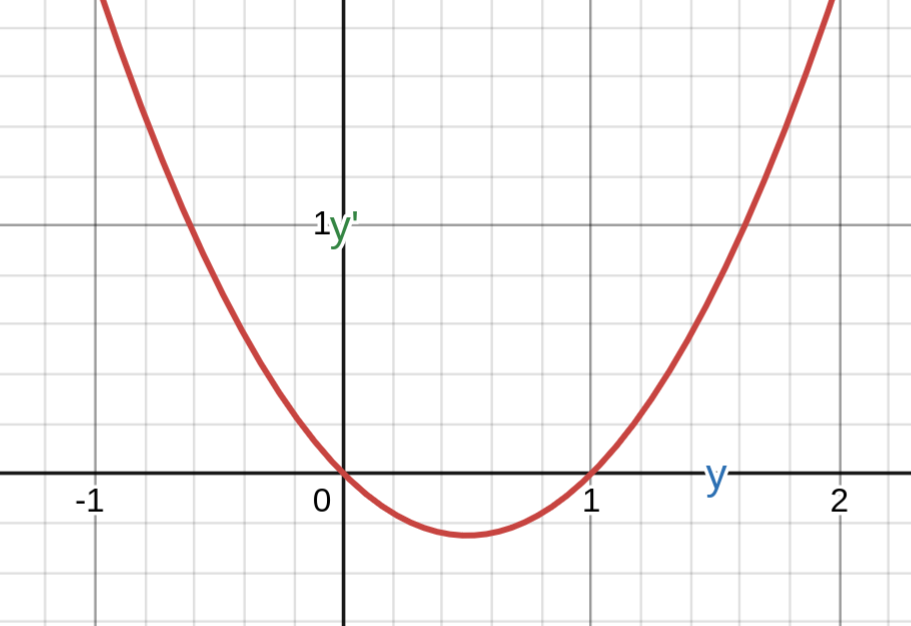
\includegraphics[width=3in]{resources/tutorial-07-phase1.png}
    \end{center}

    Let $y(t)$ be a solution to this differential equation.

    \begin{enumerate}
        \item When $y(t)=1.5$, is $y$ increasing or decreasing? 
        \item When $y(t)=0.5$, is $y$ increasing or decreasing?
        \item Are there values of $y$ for which $y$ is neither increasing nor decreasing? What are these values called? (\emph{Hint: it starts with an ``E''.})
        \item If $y(0)=0.5$, predict what $y(100)$ will be. How did you arrive at your predication?
    \end{enumerate}

    \item Consider the below ODEs and problem descriptions. Match each ODE to a problem description and justify your answer.
    \begin{tcolorbox}[sharp corners=all,colframe=tolGrey,colback=white]
        \begin{multicols}{2}
        \begin{enumerate}[label={(\roman{enumii})},nosep,itemsep=1mm]
            \item $y'=ky$
            \item $y'=ky(M-y)$
            \item $y'=\frac{ky}{\sqrt{t+1}}$
        \end{enumerate}
        \end{multicols}
    \end{tcolorbox}

    Consider the below descriptions:
    \begin{enumerate}
        \item Babies are born on an island at a rate proportional to the total population, but there is a carrying capacity which limits the number of people that the island can support.
        \item Babies are born on an island at a rate proportional to the total population.
        \item Babies are born on an island at a rate prportional to the total population, but as time progresses, people become richer, lazier, and have fewer children.
    \end{enumerate}



    \item Consider the differential equation for an autonomous ODE $y'=f(y)$.
    Your job is to graph a function $f$ so that the corresponding ODE:
    \begin{itemize}[nosep]
        \item has three equilibria;
        \item has at least one stable equilibrium; and
        \item \textbf{NONE} of the equilibria are unstable.
    \end{itemize}

    After you make your plot:
    \begin{enumerate}
        \item Explain/justify why your sketch ensures each of the above properties.
        \item Make a rough sketch of each \emph{qualitatively different} 
        solution to your ODE. E.g., an always increasing concave-up solution would be different from an always increasing concave-down solution, etc..
    \end{enumerate}
\end{enumerate}
